\documentclass[]{article}   % list options between brackets
\usepackage{amsmath}        % list packages between braces
\usepackage[utf8]{inputenc}
\usepackage{graphicx}
\usepackage{lmodern}

%Page
\addtolength{\oddsidemargin}{-.875in}
\addtolength{\evensidemargin}{-.875in}
\addtolength{\textwidth}{1.75in}
\addtolength{\topmargin}{-.875in}
\addtolength{\textheight}{1.75in}
%Page

% type user-defined commands here
\begin{document}

\title{Études et expérimentation de la reconnaissance des chiffres}   % type title between braces
\author{NGUYEN Van Tho - NGUYEN Quoc Khai}         % type author(s) between braces
\date{22 Décembre, 2013}    % type date between braces
\maketitle

\section{Introduction}
Dans ce TP, nous visons à développer un programme qui peut reconnaître des chiffres. Pour 
il existe plein de recherches qui donnent les résultats efficaces 
tels que K-plus proches voisins, Décision stumps, Classification non linéaire, SVMs, 
Réseaux neuraux et Réseaux de convolution\cite{c1}. Il existe aussi des méthode moins 
efficace comme Classification linéaire, la classification bayésienne. Pour 
trouver des bonnes méthodes, nous examinons quelques algorithmes qui rendent des 
résultats acceptables et qui sont faisables. Après ces études, nous avons choisit 2 
méthodes, K-plus proches voisins et SVM. Nous expérimentons plusieurs paramètres de ces 
deux méthodes pour trouver la meilleure configuration.\\

\section{Descriptions des méthodes utilisées}
Dans ce TP, nous avons utilisé 2 méthodes, K-plus proches voisins et SVM
\subsection{K-plus proches voisins Euclide}
Cette méthode est réalisé dans des étapes suivantes.
\subsubsection{Détection des blocks}
Chaque image est divisée en N blocks de même taille. On vous signale que le choix du nombre de block est si important, cela influence beaucoup au résultat de reconnaissance. Après avoir testé des paramètres, on a choisi de mettre $N = 14x14 = 196$.
\subsubsection{Calcul du descripteur}
Un descripteur contient $N$ éléments et une valeur d'un élément $e$ est la somme des pixels d'un block qu'on a détecté dans la dernière étape.
\subsubsection{Calcul de la distance d'Euclide entre deux descripteurs}
\begin{equation}
D = \sqrt{\sum_{\substack{
   	(1<=i<=N)}} (e_{1i} - e_{2i})^2}
\end{equation}
\subsubsection{K-plus proches voisins (K-Nearest Neighbors)}
Quand on entre une image de test, le programme calcule la distance $D$ entre cette image avec toutes les images d'apprentissage, ils donnes $K$ images ayant les distances les plus courtes. Choix du type le plus populaire pour le type de l'image de test. Ici, K est un paramètre d'entré. En observant le résultat des tests, nous trouvons que $K = 4$ donne le meilleur résultat.
\subsection{Méthode SVM}
Nous avons aussi implémenté un programme utilisé la méthode SVM. Cette méthode utilise la 
même structure que la méthode K-plus proches voisins. Autrement dit, l'image est divisée 
en N bloques. Le vecteur caractéristique est un vecteur de taille N, chaque élément de 
vecteur est la somme des valeurs de niveau de gris d'un bloc. 

Dans ce travail, nous avons utilisé l'implémentation de SVM de OpenCV.

\begin{center}
 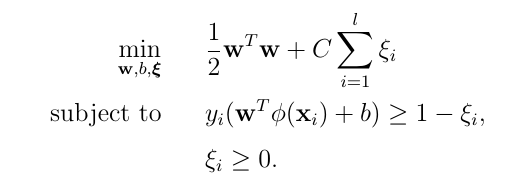
\includegraphics{./images/svm.png}
\end{center}

Le kernel gaussien utilisé dans notre programme:
\begin{center}
$K(x_{i}, x_{j}) = exp(-\gamma(x_{i}- x_{j})^2)$
\end{center}

\section{Présentation du programme}
Ce programme contient 4 classes divisées en 8 fichiers : \textit{channel.h channel.cpp IO.h IO.cpp training.h training.cpp control.h et control.cpp} et un fichier de la fonction \textit{main}, \textit{main.cpp}. Un \textit{makefile} sert à faciliter de compiler le programme.

Ce programme a les fonctionnalités suivantes :
\begin{enumerate}
\item Création des descripteurs pour les images d'apprentissage ou de test et les enregistre dans un fichier.
\item A partir de deux fichiers de descripteur de test et d'apprentissage, le programme catégorise les images vers la catégorie correspondante.
\end{enumerate}

Dans ce programme, aucun algorithme est réutilisé. Par contre, nous avons utilisé la librairie OpenCV pour le traitement de base.
\section{Expérimentation}
\subsection{Évaluation}
Pour évaluer le programme, nous avons utilisés deux critères: le taux de précision et le 
temps de calcul. Une configuration des paramètres est considérée meilleure si elle rend 
un résultat avec un grand taux de précision et avec un petit temps de calcul.

\subsection{SVM}
Une des difficultés de l'algorithme SVM est comment choisir les bonnes paramètres. 
Un mauvais choix de paramètres peut rendre un résultat très mauvais. Avec un kernel 
gaussien, on a deux paramètres à optimiser: la constance C et le gamma. Donc, pour 
trouver les valeurs optimales de ces paramètres, nous utilisons la méthode Grid search 
proposé par Chih-Wei Hsu, Chih-Chung Chang et Chih-Jen Lin \cite{c2}.En effet, nous avons 
expérimenté les valeurs de C de $2^{-5}$ à $2^{15}$ et gamma de $2^{-19}$ à $2^3$. De 
plus, pour trouver le nombre optimal de blocs, nous expérimenté plusieurs nombre de bloc:
de 7 à 16.

Les bonnes valeurs de C reçues sont de 2 à 8. Les bonnes valeurs de gamma sont de 0.0001 
à 0.008. Nous avons fait la deuxième série d'expérimentation avec ces valeurs de C et 
gamma.

\subsection{Méthode KNN}
Avec cette méthode, pour obtenir le bon résultat, il faut bien choisir des paramètres 
comme le nombre de block, le K plus proches voisins.
\begin{enumerate}
\item Nombre de block, ce paramètre est important. Quand le nombre de block est petit, le 
résultat n'est pas exact. Par contre, quand on le met très grand, la méthode peut se 
tromper aussi à cause des bruits dans les images.
\item K plus proches voisins, cette paramètre est aussi importante mais c'est plus facile 
de fixer cette paramètre. Par rapport des testes, nous trouvons que le bon est d'entre 1 
et 5.
\end{enumerate}
\section{Analyse des résultats obtenus}
\subsection{Méthode KNN}

\begin{figure}[!htb]
\minipage{0.55\textwidth}
  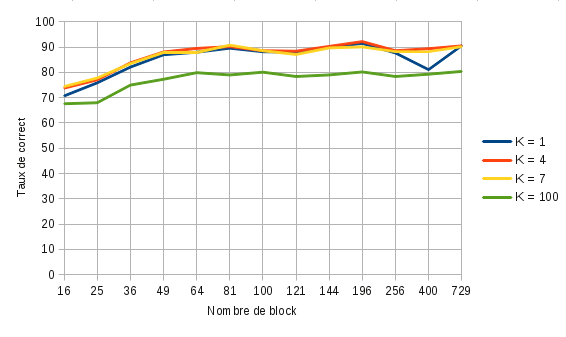
\includegraphics[width=\linewidth]{images/graphique.png}
  \caption{Taux de correct}\label{fig:awesome_image2}
\endminipage\hfill
\minipage{0.55\textwidth}
  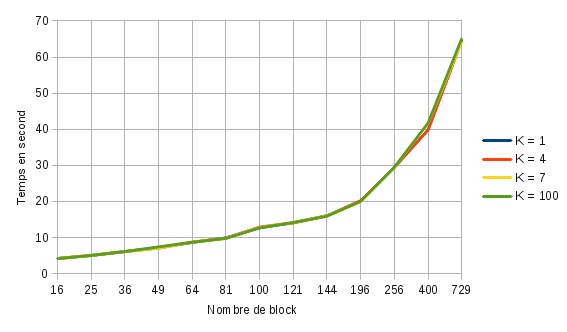
\includegraphics[width=\linewidth]{images/graphique1.png}
  \caption{Temps de calcul}\label{fig:awesome_image3}
\endminipage\hfill
\end{figure}

\subsection{Méthode SVM}
Comme nous avons discuté dans la section expérimentation, le point crucial de cette 
méthode est de bien choisir la configuration de C et gamma. Voir les figures de 
résultats, on constate qu'il y a un petit compromis entre le taux de précision et le 
temps de calcul. En fait, quand le résultat est crucial, on peut utiliser la 
configuration avec C = 3, gamma = 0.002 et le nombre de blocs est 14x14. Cette 
configuration rend le taux de précision de 
94.8\% et le temps de calcul est 4 seconds.
Par contre,quand le temps de calcul est plus crucial, la configuration avec C = 8, gamma = 
0.0004 le nombre de blocs est 7x7. Cette configuration rend le taux de précision de 
92.1\% et le temps de calcul est 0.8 seconds. 

\pagebreak
\begin{figure}[!htb]
\minipage{0.55\textwidth}
  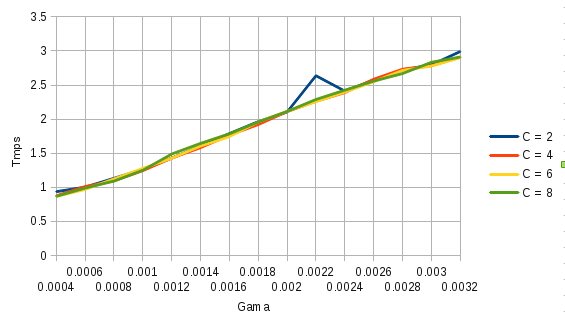
\includegraphics[width=\linewidth]{images/graphique2.png}
  \caption{Taux de correct, blocs = 7x7}\label{fig:awesome_image2}
\endminipage\hfill
\minipage{0.55\textwidth}
  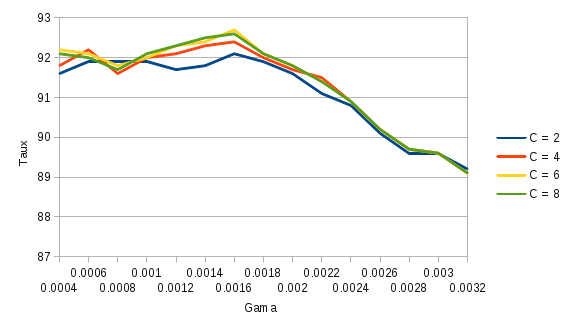
\includegraphics[width=\linewidth]{images/graphique3.png}
  \caption{Temps de calcul, blocs = 7x7}\label{fig:awesome_image3}
\endminipage\hfill
\end{figure}

\begin{figure}[!htb]
\minipage{0.5\textwidth}
  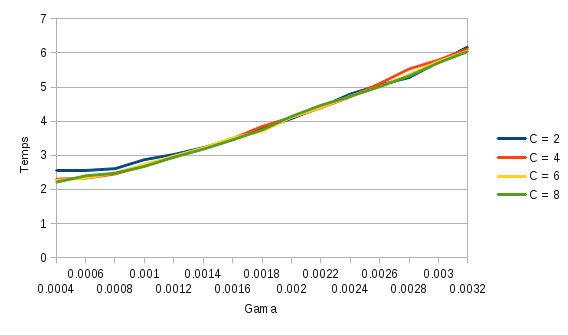
\includegraphics[width=\linewidth]{images/graphique4.png}
  \caption{Taux de correct, blocs = 14x14}\label{fig:awesome_image2}
\endminipage\hfill
\minipage{0.5\textwidth}
  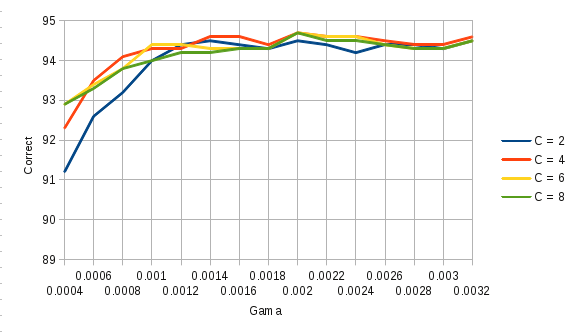
\includegraphics[width=\linewidth]{images/graphique5.png}
  \caption{Temps de calcul, blocs = 14x14}\label{fig:awesome_image3}
\endminipage\hfill
\end{figure}

\subsection{Comparaison entre KNN et SVM}
Nous constatons que la méthode SVM peut donner des résultats beaucoup plus vite que la 
méthode KNN. De plus, la précision de résultat rendu par SVM est un peu importante par 
rapport à celui rendu par la méthode KNN.



\section{Conclusion}
Dans ce projet, nous avons implémenté deux algorithmes pour la reconnaissance de chiffres 
manuscrit. Nous avons aussi expérimenté plusieurs configurations des paramètres pour 
trouver la meilleure configuration.

En général, la méthode SVM est meilleure que la méthode KNN en toutes les termes 
d'évaluation. Cependant, pour trouver les bonnes paramètres, on doit faire plus 
d'expérimentation.

\clearpage
\begin{thebibliography}{9}
\bibitem{c1}
  David Lowe
  \emph{THE MNIST DATABASE of handwritten digits}.
  Yann LeCun, Courant Institute, NYU,
  Corinna Cortes, Google Labs, New York,
  Christopher J.C. Burges, Microsoft Research, Redmond,
  \emph{http://www.cs.ubc.ca/~lowe/keypoints/}
   
\bibitem{c2}
  Chih-Wei Hsu, Chih-Chung Chang, and Chih-Jen Lin
  \emph{A Practical Guide to Support Vector Classification}.
  Department of Computer Science
National Taiwan University, Taipei 106, Taiwan
  \emph{http://www.csie.ntu.edu.tw/~cjlin}
 
\end{thebibliography}

\end{document}